\documentclass{article}
\usepackage{tikz}
\usetikzlibrary{math} % LATEX and plain TEX when using TikZ
\begin{document}
%\begin{tikzpicture}
\tikzmath{
	% Adapted from http://www.cs.northwestern.edu/academics/courses/110/html/fib_rec.html
	function fibonacci(\n) {
		if \n == 0 then {
			return 0;
		} else {
			return fibonacci2(\n, 0, 1);
		};
	};
	function fibonacci2(\n, \p, \q) {
		if \n == 1 then {
			return \q;
		} else {
			return fibonacci2(\n-1, \q, \p+\q);
		};
	};
	int \f, \i;
	for \i in {0,1,...,20}{
		\f = fibonacci(\i);
		print {\f, };
	};
}
%\end{tikzpicture}
\tikz[x=0.25cm,y=0.25cm,
evaluate={
	int \i, \j;
	for \i in {0,...,10}{
		for \j in {0,...,10}{
			\a{\i,\j} = (\i+\j)*5;
		};
	};
}
]
\foreach \i in {0,...,10}
\foreach \j in {0,...,10}
\fill [red!\a{\i,\j}!yellow] (\i,\j) rectangle ++(1, 1);

\tikzmath{
	int \x, \y;
	\y = 0;
	for \x1 in {1,...,5}{
		for \x2 in {10,20,...,50}{
			\y = \y+\x1*\x2;
		};
	};
}
$x_1=\x1, x_2=\x2, y=\y$

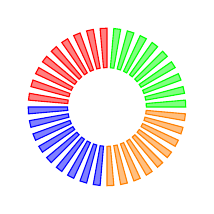
\begin{tikzpicture}
\tikzmath{
	int \x;
	for \k in {0,10,...,350}{
		if \k>260 then { let \c = orange; } else {
			if \k>170 then { let \c = blue; } else {
				if \k>80 then { let \c = red; } else {
					let \c = green; }; }; };
		{
			\path [fill=\c!50, draw=\c] (\k:0.5cm) -- (\k:1cm) --
			(\k+5:1cm) -- (\k+5:0.5cm) -- cycle;
		};
	};
}
\end{tikzpicture}

\tikzmath{
	function product(\x,\y) {
		return \x*\y;
	};
	int \i, \i, \k;
	\i = random(1,10);
	\j = random(20, 40);
	\k = product(\i, \j);
	print { $\i\times \j = \k$ };
}

\tikzmath{
	int \x, \y, \z;
	\x = random(2, 5);
	for \y in {0,...,6}{
		\z = \x^\y;
		print {$\x^\y=\z$, };
	};
}

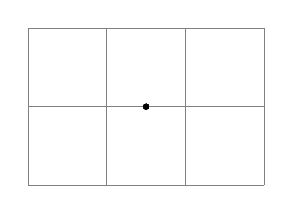
\begin{tikzpicture}
\draw [help lines] grid (3,2);
\tikzmath{
	coordinate \c;
	for \x in {0,10,...,360}{
		\c = (1.5cm, 1cm) + (\x:1cm and 0.5cm);
		{ \fill (\c) circle [radius=1pt]; };
	};
}
\end{tikzpicture}
\end{document}